\documentclass[../notes.tex]{subfiles}

\pagestyle{main}
\renewcommand{\chaptermark}[1]{\markboth{\chaptername\ \thechapter\ (#1)}{}}
\setcounter{chapter}{8}

\begin{document}




\chapter{Surface Structure and Catalysis}
\section{Surface Structure and Catalysis}
\begin{itemize}
    \item \marginnote{5/23:}Final exam:
    \begin{itemize}
        \item Single sheet with problems on both sides and a blank piece of paper to write answers on.
        \item Total time: 50 minutes.
        \item We only need to look into the specific subchapters in the final exam outline.
        \item The computation problem will be from either PSet 5 or 6.
        \item 7 true/false problems on concepts from the chapters specified in the outline.
        \item 2 true/false problems relative to plots that have been drawn in class or otherwhere.
        \item Relatively easy compared to the midterm.
    \end{itemize}
    \item Review of last lecture.
    \item The Langmuir adsorption isotherm implies rate laws for surface-catalyzed gas-phase reactions.
    \begin{itemize}
        \item Consider the surface catalysis of the first-order gas-phase reaction
        \begin{equation*}
            \ce{A(g) ->[$k_\text{obs}$] B(g)}
        \end{equation*}
        \item The observed rate law is given by
        \begin{equation*}
            \dv{\cnc{B}}{t} = k_\text{obs}P_{\ce{A}}
        \end{equation*}
        \item Assume that this reaction occurs by the following two-step mechanism.
        \begin{equation*}
            \ce{A(g)} \xRightarrow{k_a} \ce{A(ads)} \xRightarrow{k_1} \ce{B(g)}
        \end{equation*}
        \item The rate law for this mechanism is
        \begin{equation*}
            \dv{\cnc{B}}{t} = k_1\cnc{A(ads)} = k_1\sigma_{\ce{A}}
        \end{equation*}
        where $\sigma_{\ce{A}}=\sigma_0\theta$.
    \end{itemize}
    \item Derivation.
    \begin{itemize}
        \item We have that
        \begin{equation*}
            \frac{1}{\theta} = 1+\frac{1}{K_c\cnc{A}}
        \end{equation*}
        so
        \begin{equation*}
            \dv{\cnc{B}}{t} = k_1\frac{\sigma_0K_c\cnc{A}}{1+K_c\cnc{A}}
            = k_1\frac{\sigma_0bP_{\ce{A}}}{1+bP_{\ce{A}}}
        \end{equation*}
        where we have defined $b=K_c/\kB T$.
        \item At low gas pressures, $bP_{\ce{A}}\ll 1$. Here, the rate law becomes first order in reactant pressure.
        \begin{equation*}
            \dv{\cnc{B}}{t} = k_1\sigma_0bP_{\ce{A}}
            = k_\text{obs}P_{\ce{A}}
        \end{equation*}
        \item At high pressure, $bP_{\ce{A}}\gg 1$. Here, the rate law becomes zero order in reactant pressure.
        \begin{equation*}
            \dv{\cnc{B}}{t} = k_1\sigma_0
            = k_\text{obs}
        \end{equation*}
    \end{itemize}
    \item Most reactions are studied at low pressure and the observed rate constant is equal to the product $k_1\sigma_0b$.
    \item Relation to enzyme catalysis.
    \begin{itemize}
        \item There, we formed an enzyme-substrate complex, which then decomposed.
        \item Here, we form a substrate-adsorption complex that then decomposes.
        \item In surface catalysis, we refer to our surface as the substrate. It's a lattice on which our reaction happens.
        \item For enzyme catalysis, we learned that the rate has a linear dependence on substrate concentration for small $\cnc{S}$ and no dependence for big $\cnc{S}$.
        \item Recall that the Michaelis-Menten mechanism is a reaction mechanism for enzyme catalysis.
        \begin{itemize}
            \item It predicts our first $\to$ zero order substrate concentration dependence change.
            \item It also comes packaged with the Lineweaver-Burk plot.
        \end{itemize}
    \end{itemize}
    \item The surface structure is different from that of the bulk.
    \item Surface characterization tools.
    \begin{itemize}
        \item Scanning electron microscopy (SEM).
        \begin{itemize}
            \item A scanning electron microscope (SEM) is a type of electron microscope that produces images of a sample by scanning the surface with a focused beam of electrons. The electrons interact with atoms in the sample, producing various signals that contain information about the surface topography and composition of the sample.
            \item There's also transmission, that detects electrons which pass through the surface.
        \end{itemize}
        \item Low-energy electron diffraction (LEED).
        \begin{itemize}
            \item Electrons with kinetic energies in the range of \SIrange{5000}{10000}{\kilo\joule\per\mole} are commonly called low-energy electrons and penetrate the surface of a metal to only about \SI{500}{\pico\meter}.
        \end{itemize}
    \end{itemize}
    \item The surfaces have many types of defects.
    \begin{figure}[h!]
        \centering
        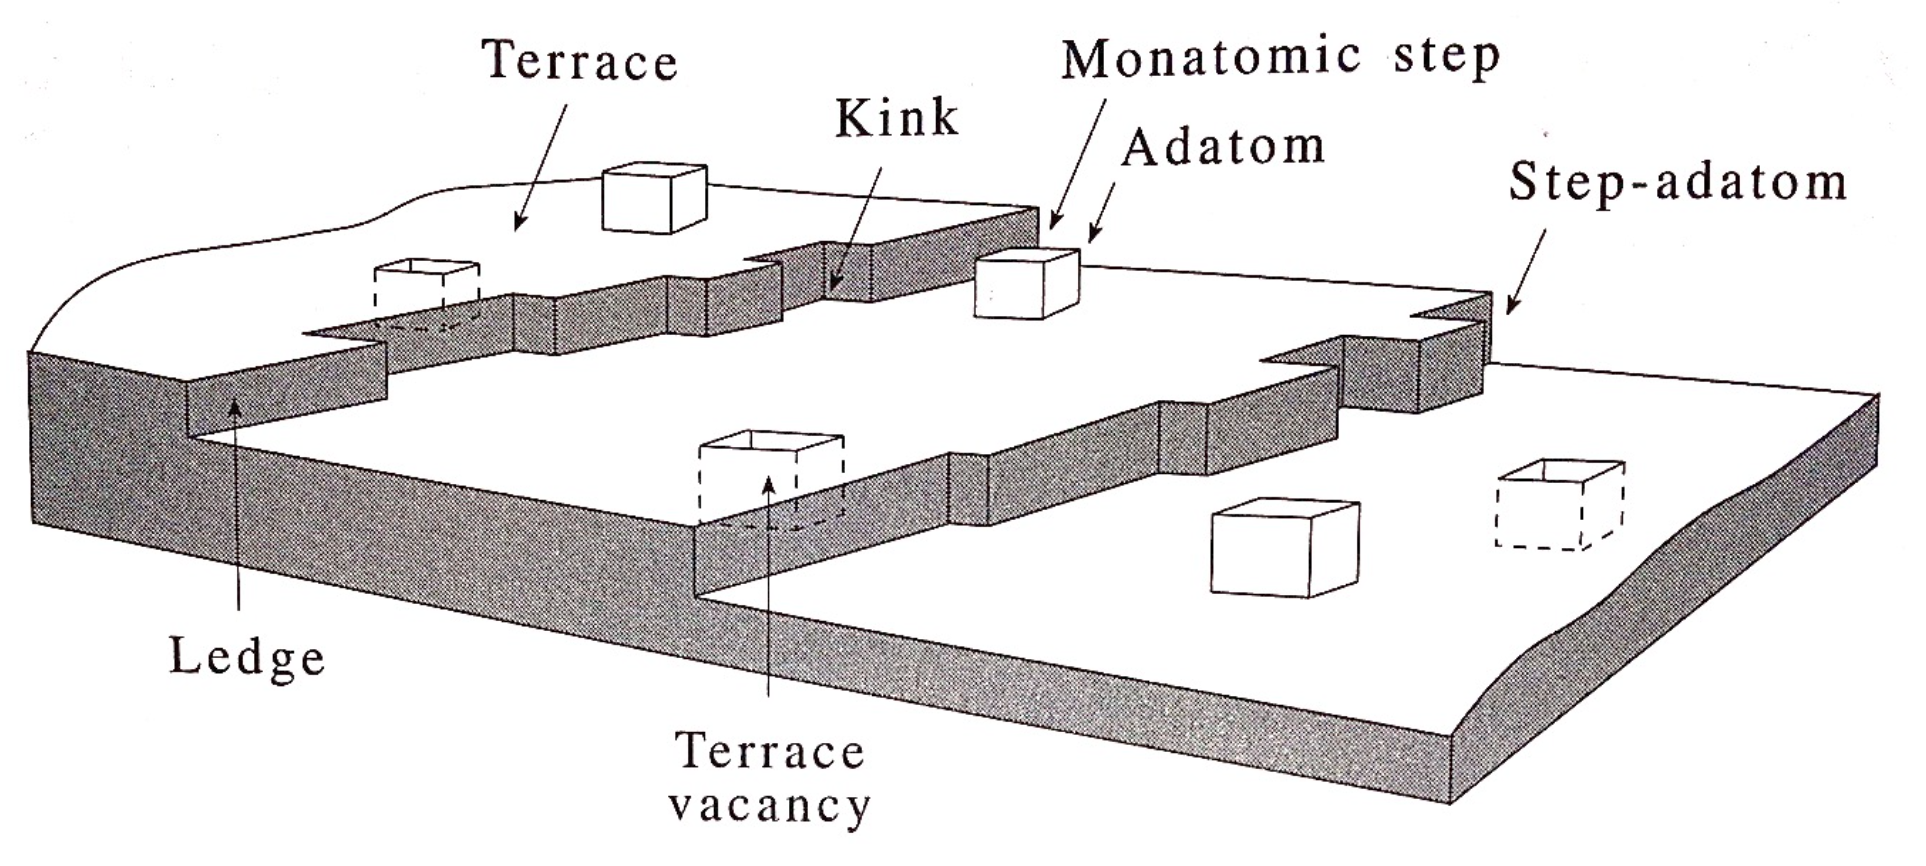
\includegraphics[width=0.6\linewidth]{../ExtFiles/surfaceDefects.png}
        \caption{Surface features and defects.}
        \label{fig:surfaceDefects}
    \end{figure}
    \begin{itemize}
        \item An illustration of some of the possible structural defects that occur on a surface. The surface is characterized by ledges, steps, and terraces.
        \item The steps can be one or many rows of atoms. The steps also need not be straight, which gives rise to kinks.
        \item Single atoms (or \textbf{adatoms}) may sit anywhere on a terrace.
        \item There can also be vacancies on the terrace, leaving small holes in the surface. These holes are indicated by dotted cubes.
        \item The defects are often some of the active sites.
        \begin{itemize}
            \item The locations of the defects are locations where the surface energy is high. These high energy spots become sweet spots for reactions. Molecules will come in, bind to that high energy site, and use the energy to form a product.
        \end{itemize}
        \item Doping.
        \begin{itemize}
            \item $p$-type doping of semiconductors can introduce holes. $n$-type doping of semidonductors introduces electrons.
        \end{itemize}
        \item Defect types.
        \begin{itemize}
            \item We can have hole defects, line defects, and plane defects.
            \item Some defects can be bad, degrading the whole material, but in catalysis, they're good.
        \end{itemize}
    \end{itemize}
    \item The reaction between \ce{H2} and \ce{N2} to produce \ce{NH3} can be surface catalyzed.
    \begin{equation*}
        \ce{3H2(g) + N2(g) -> 2NH3(g)}
    \end{equation*}
    \begin{itemize}
        \item Mechanism.
        \begin{align*}
            \ce{H2(g) + 2S(s)} &\Longleftrightarrows \ce{2H(ads)}\\[-1.6em]
            \ce{N2(g)} &\Longleftrightarrows \ce{N2(ads)}\\[-1.6em]
            \ce{N2(ads) + 2S(s)} &\Longleftrightarrows \ce{2N(ads)}\\[-1.6em]
            \ce{N(ads) + H(ads)} &\Longleftrightarrows \ce{NH(ads)}\\[-1.6em]
            \ce{NH(ads) + H(ads)} &\Longleftrightarrows \ce{NH2(ads)}\\[-1.6em]
            \ce{NH2(ads) + H(ads)} &\Longleftrightarrows \ce{NH3(ads)}\\[-1.6em]
            \ce{NH3(ads)} &\Longleftrightarrows \ce{NH3(g)}\\[-1.6em]
        \end{align*}
        \begin{itemize}
            \item Splitting nitrogen is the hardest part.
            \item The second step is physisorption.
            \item The third step is dissociative chemisorption.
        \end{itemize}
        \item The relative rates of ammonia synthesis for different transition metal catalysts can be plotted.
        \begin{itemize}
            \item The shape of the plotted data is influenced by the opposing effects of the strength of the surface nitrogen bond and the activation energy of the dissociative chemisorption of \ce{N2}.
        \end{itemize}
    \end{itemize}
    \item Summary of what's essential in Chapter 31.
    \begin{itemize}
        \item Miller indices and drawing the planes to which they correspond.
        \begin{itemize}
            \item If we only need to draw one on the exam, skip the one through the origin and draw the next one.
        \end{itemize}
        \item The total scattering intensity (e.g., from the homework).
        \item Isotherms.
        \begin{itemize}
            \item We need to be clear about the information that the Langmuir plot can give us.
        \end{itemize}
    \end{itemize}
    \item Tian leaves the door open for us to reach out to him in the future.
    \item Also don't worry about the midterm too much; Tian will try to adjust in the best possible way.
\end{itemize}



\section{Chapter 31: Solids and Surface Chemistry}
\emph{From \textcite{bib:McQuarrieSimon}.}
\begin{itemize}
    \item \marginnote{5/24:}\textcite{bib:McQuarrieSimon} covers the derivation of rate laws for surface-catalyzed reactions from class.
    \item \textcite{bib:McQuarrieSimon} derives rate laws for bimolecular gas-phase reactions occurring via the \textbf{Langmuir-Hinshelwood mechanism} and \textbf{Eley-Rideal mechanism}.
    \item \textcite{bib:McQuarrieSimon} covers surface structure, including SEM and LEED.
    \item The activation barrier in nitrogen fixation is so high (owing to the BDE of \ce{N2}) that even though the reaction is exothermic, the reactant molecules can be stored together forever with no reaction ever taking place.
    \begin{itemize}
        \item On an iron surface, however, the BDE of \ce{N2} is approximately \SI{10}{\kilo\joule\per\mole}.
    \end{itemize}
    \item \textbf{Volcano curve}: A plot with a linear ascent and descent.
    \item An example is the plot of the relative rates of ammonia synthesis for different transition metal catalysts, which peaks in the middle.
    \begin{itemize}
        \item The two forces at play in this particular plot are an increase in $d$ electrons decreasing the strength of the metal-nitrogen bond in adsorbed \ce{NH3} molecules, and an increase in $d$ electrons increasing the \ce{N2} BDE.
    \end{itemize}
    \item Surface orientation also affects reaction rate: A smooth 110 surface gives rise to a negligible yield of ammonia, while a rough 111 surface has the highest yield.
    \begin{itemize}
        \item This particular result steps from changes in the BDE of \ce{N2} across the types of surfaces.
    \end{itemize}
\end{itemize}




\end{document}